\documentclass[12pt]{jarticle} 
%\documentstyle[12pt,fleqn,epsf,iepaper,cite]{jarticle}
%\documentstyle[12pt,iepaper,eclepsf,oddchar]{jarticle}
\usepackage[dvipdfm]{graphicx}
\usepackage{iepaper}
\usepackage{epsf}
\usepackage{ccaption}
\usepackage{algorithm}
\usepackage{algorithmic}
\usepackage{subcaption}
\usepackage{enumerate}
\usepackage{comment}
\usepackage{url}
\usepackage{multirow}
\usepackage{diagbox}
\usepackage{amssymb}
\usepackage{mathtools}
\usepackage{wrapfig}
\usepackage{graphicx}
\usepackage{float}
\usepackage{amsmath}
\usepackage{lipsum}
\usepackage[jis2004]{otf}

\title{深層強化学習に基づく
\par
トレーディングカードゲーム環境の構築}
\author{西村 昭賢} 
\gakuseki{1201201100}[B]  %卒論はB,修論はM
\group{第 1 研究グループ}            % 卒論の場合
\shidou{森 直樹 教授}                          % 卒論の場合
%\syusa{教授}                            % 修論の場合
%\hukusa{教授}{教授}

%図番号を「(section番号).(図番号)」とするため
\makeatletter
 \renewcommand{\thefigure}{%
   \thesection.\arabic{figure}}
  \@addtoreset{figure}{section}
\makeatother

\makeatletter
 \renewcommand{\thetable}{%
   \thesection.\arabic{table}}
  \@addtoreset{table}{section}
\makeatother

\makeatletter
 \renewcommand{\theequation}{%
   \thesection.\arabic{equation}}
  \@addtoreset{equation}{section}
\makeatother


\begin{document} 
\maketitle 
\pagenumbering{roman} 
%%% 目次
\tableofcontents
\newpage
%
%% 図一覧
\listoffigures
\newpage 

%% 表一覧
 \listoftables
 \newpage

\pagenumbering{arabic} 

% 文書開始
\newpage
\changeindent{0cm}
\section{はじめに}
\changeindent{2cm}

近年, 人工知能に関する研究分野は目覚ましい発展を遂げており様々な分野に応用されている. その中でも人間の学習プロセスに近いとされる強化学習と深層学習を融合した深層強化学習は自動運転やロボット, 推薦システム等の実生活の問題解決への応用例が数多く報告されている \cite{Vehicle}\cite{robotics}\cite{recommendation}. 
実世界の問題解決への応用だけでなく, 深層強化学習はゲームへの応用も盛んである.
特に将棋や囲碁といった, プレイヤーが意思決定をする段階でそれ以前の意思決定の過程がすべて把握可能な完全情報ゲームへの応用においては AlphaGo \cite{AlphaGo}, AlphaZero \cite{AlphaZero} を筆頭に現役のプロプレイヤーを圧倒する性能を残しており成果が顕著である. 
最近では麻雀やポーカーのような, プレイヤーに与えられる情報が部分的である不完全情報ゲームへの応用も注目されている.
\par
本研究では不完全情報ゲームであるトレーディングカードゲーム環境への深層強化学習の適用と深層強化学習を用いたゲームバランス調整手法を提案し, 独自に構築したトレーディングカードゲーム環境を用いて数値実験することでその有効性を示す. 
\par
以下に本論文の構成を示す.  まず, 2 章では本研究で用いる要素技術について, 3 章では類似研究と提案手法について説明する. 4 章では本環境で独自に構築したトレーディングカードゲーム環境の概要を示す. 5 章で実験方法の説明をし, 6 章で実験結果と考察を示す. そして, 7 章に本研究のまとめ及び今後の課題について述べる.
\clearpage

\section{要素技術}

\subsection{OpenAI Gym}
OpenAI Gym \cite{OpenAIGym} は非営利企業 OpenAI が提供する強化学習のシミュレーション用ライブラリであり, 強化学習の環境として図 \ref{fig:OpenAIGymSample} に示すように多くのゲーム, シミュレータが登録されている. さらには提供されているインターフェースに沿って, エージェントの行動空間や状態空間, 報酬などを定義,実装することで独自の強化学習環境を構築し利用することができる. また, 様々な強化学習用ライブラリに対応しているため比較的容易に強化学習を試すことができる.

\begin{figure}[ht]
  \centering
  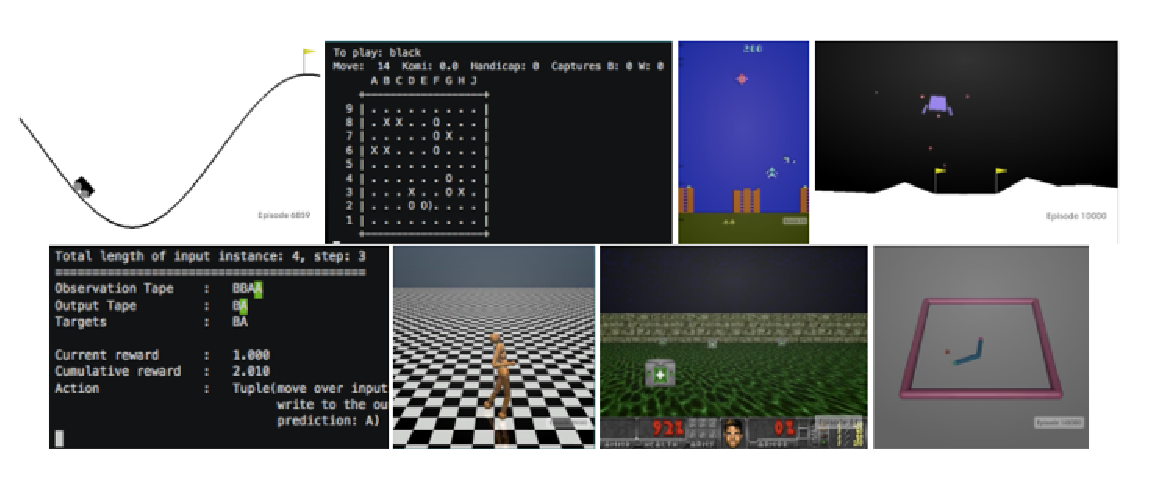
\includegraphics[width=150mm]{assets/OpenAiGym.eps}
  \vspace{-0.3cm}
  \caption{OpenAI Gym が提供している様々な学習環境}
  \label{fig:OpenAIGymSample}
\end{figure}



\subsection{Q 学習}
強化学習では,エージェントが行動することで環境における状態が変化し報酬を得る. 強化学習における行動はその直後に獲得する報酬の大きさではなく, 未来に渡っての報酬の総和を見積もった値である「価値」の最大化に繋がるかという観点で評価される.
価値の最大化を目指す場合にはある状態 $s$ において行動 $a$ をとった時の価値が分かればよい.この価値のことを Q 値, あるいは行動価値関数と呼ぶ. この Q 値を基に行動を選択していく価値ベースの強化学習手法において代表的な手法が Q 学習である. 
 Q 学習ではエージェントの 1 ステップごとに (\ref{updateQ}) 式に示す更新式で Q 値を更新する.
\begin{equation}
  \centering
  \label{updateQ}
  Q(s_t,a_t) \leftarrow Q(s_t,a_t) + 
   \alpha(r_{t+1} + \gamma \mathrm{max}_{a_{t+1}}Q(s_{t+1},a_{t+1}) - Q(s_t,a_t))
\end{equation}
なお $t$ は時間, $r$ は報酬, $\alpha$ は Q 値の更新度合いを表す学習率, $\gamma$ は将来の価値の割引度合いを表す割引率である. 
\par
また, Q 学習に代表される強化学習においては環境の調査を目的とする探索と, 探索により得られた良い報酬を得ることができる経験の活用をそれぞれどの程度にすればよいかといういわゆる「探索と活用のトレードオフ」という問題が発生する. これを解決する手法として一般的なものが $\mathrm{\epsilon - greedy}$ 法である. $\mathrm{\epsilon - greedy}$ 法では確率 $\epsilon$ でランダムに行動し探索, それ以外では Q 値が最も高い行動を選択することで探索と活用のバランスをとっている.  


\subsection{Deep Q Network}
Q 学習を実際に実装する場合, 状態と行動をインデックスとした Q 値のテーブルを作成する. しかし状態空間や行動空間が高次元である, あるいは状態や行動が離散値ではなく連続値で表現される場合には Q テーブルのメモリ量は爆発してしまう. この問題を解決した技術が Deep Q Network (DQN) \cite{DQN} である.
 DQN ではニューラルネットワークを用いて, ある状態における行動ごとの Q 値を推定することでたとえ状態が連続値であっても学習可能としている.
 \par
 DQN では, 主に Experience Replay と呼ばれる工夫により深層学習を用いても安定な学習を可能としている. 
 Experience Replay はエージェントが経験した過去の体験を Replay Memory に一定期間保存しておき, 過去の遷移情報をランダムにサンプリングして学習することでデータの偏りを無くす手法である. この時の遷移情報は状態 $s_i$ において行動 $a_i$ を選択した時, 報酬 $r_i$ を獲得し状態 $s_{i+1}$ に遷移したという情報を $(s_i, a_i, r_i, s_{i+1})$ とまとめて記憶する. \par
 DQNの疑似コードを \ref{alg:DQN} に示す.
 \begin{figure}[H]
  \begin{algorithm}[H]
      \caption{
        deep Q-learning with experience replay
        }
      \begin{algorithmic}[1] 
      \STATE Initialize replay memory $D$ to capacity $N$
      \STATE Initialize action-value function $Q$ with random weights $\theta$
      \STATE Initialize target action-value function $\hat{Q}$ with weights $\theta^{-}$ = $\theta$
      \FOR{episode = 1, $M$} 
      \STATE Initialize sequence $s_{1} = \{x_1\}$ and preprocessed sequence $\phi_1$ = $\phi(s_1)$ 
      \FOR{$t$ = 1, $T$}
      \STATE With probability $\epsilon$ select a random action $a_{t}$
      \STATE otherwise select $a_t = \mathrm{argmax}_{a}Q(\phi(s_{t}),a; \theta)$
      \STATE Execute action $a_t$ in emulator and observe reward $r_t$ and image $x_{t+1}$
      \STATE Set $s_{t+1} = s_t,a_t,x_{t+1}$ and preprocess $\phi{t+1} = \phi(s_{t+1}) $
      \STATE Store transition $(\phi_t,a_t,r_t,\phi_{t+1})$ in $D$
      \STATE Sample random minibatch of transitions $(\phi_j,a_j,r_j,w_{j+1})$ from $D$
      \STATE Set $y_j = $ $\left\{
        \begin{aligned}
            &r_j \quad & \text{if episode terminates at step } j + 1 \\
            &r_j + \gamma \mathrm{max}_{a'} \hat{Q}(\phi_{j+1},a';\theta^{-}) \quad  & \text{otherwise}\\
        \end{aligned}
      \right.     $   
      \STATE Perform a gradient descent step on $(y_j - Q(\phi_j,a_j;\theta))^2$ with respect to the network parameters $\theta$
      \STATE Every C steps reset $\hat{Q} = Q$
        
      \ENDFOR
      \ENDFOR
      \end{algorithmic}
  \end{algorithm}
  \caption{DQN のアルゴリズムの疑似コード \cite{DQN_algorithm}}
  \label{alg:DQN}
  \end{figure}

\subsection{Genetic Algorithm}
Genetic Alogorithm (GA) とは, 生物の進化と進化の過程を模した最適化手法であり, 主に組み合わせ最適化問題に対して適用される. GA では 1 つの解を 1 つの個体として表現し, 多数の個体からなる個体群を用いて解空間の多点を同時に探索する. 各個体はどの程度良い解であるかという指標として適用度を持つ. また, 各個体は染色体と呼ばれる配列で表される. この染色体を構成する要素を遺伝子, 染色体上の遺伝子が収まる座標を遺伝子座と呼ぶ. 探索においては, 個体群に対して選択, 交叉, 突然変異と呼ばれる 3 種類の遺伝演算子を適用させ世代と呼ばれる探索ステップを進めていく.\par
選択では, 探索において適用度が良好な個体が存在する部分を重点化するように現在の個体群から個体を選び, 次世代の個体群を生成する. 選択方法としては, 個体の適応度に比例する確率で個体を選択するルーレット戦略, 個体群からランダムに数個個体を抽出しその中で最も良好な個体を選択するトーナメント戦略がある. またこれらと併用される戦略として各世代の最良個体を保存するエリート保存戦略がある. エリート保存戦略により探索で発見した良い個体が失われることを防ぐことができる. \par
交叉では, 2 つの個体からそれらの形質を受け継いだ新たな個体を生成する. 交叉においても染色体のランダムな 1 点で染色体を切断し部分列を染色体同士で交換する 1 点交叉, ランダムな 2 点で切断する 2 点交叉, 遺伝子座ごとランダムに交換する一様交叉など様々な方法がある. \par
突然変異では, 各遺伝子座の遺伝子を許容された範囲の遺伝子の内容に置換する.
交叉や突然変異にはそれぞれ確率が設定されていることが一般的である. 



\subsection{Nondominated
Sorting Genetic Algorithm II}
Nondominated
Sorting Genetic Algorithm II (NSGA-II) とは, 与えられた制約下において複数の目的関数を最大化する多目的最適化問題を解く多目的最適化 GA の 1 つである. 一般的に多目的最適化問題においては複数の目的関数を同時に最大化する完全な最適解は存在せず, 代表的な解の概念としてパレート最適解がある. パレート最適解とは解の中で非劣解である解である. GA は個体群により解空間における多点を同時に探索するため 1 回の実行で複数のパレート最適解集合を得ることができる. このパレート最適解集合をパレートフロントと呼ぶ. \par
NSGA-II では, 真のパレートフロントへと探索を進めていく過程において個体群に高速非優越ソートを用いて解をランク付けし, このランクと後述する混雑距離に基づいて個体を選択する. また, 解の多様性を維持するためにある 1 つの解の両隣にある 2 つの解の平均距離である混雑距離と呼ばれる評価尺度を用いる.
\par
図 \ref{alg:NSGA2} にNSGA-II のアルゴリズムの概要を示す.
\begin{figure}[H]
  \begin{algorithm}[H]
      \caption{
        NSGA-II
        }
      \begin{algorithmic}[1] 
        \STATE 大きさ N の初期個体集団 P をランダムに生成する
        \STATE 非優越ソートを用いて, P の各個体にランクを付与し, 各ランク毎に属する個体に混雑距離を付与する
        \STATE P に対して, 選択, 交叉, 突然変異の遺伝子操作を施し, 大きさ N の子集団 Q を生成する
        \STATE P $\cup$ Q の各個体に対して非優越ソードでランクを付与し, 各ランク毎に属する個体に混雑距離を付与する. ランク上位 N 番目までの個体によって集団 P を構成する. なおランクが同じ個体については混雑距離が大きい個体を優先して選択する.
        \STATE 3 に戻る.
      \end{algorithmic}
  \end{algorithm}
  \caption{NSGA-II のアルゴリズムの概要 \cite{NSGA-2}}
  \label{alg:NSGA2}
  \end{figure}


\clearpage
\section{提案手法}
本研究では, 主に 3 つの手法を提案する. 以下, 各提案手法を説明する

\subsection{提案手法 1 : 数値実験用の TCG 環境}
Magic : The Gathering \footnote[1]{https://magic.wizards.com} に代表される TCG は 2 人のプレイヤーからなるゲームである. 囲碁や将棋のように, プレイヤーは先攻と後攻に分かれてターン制で進行していく. TCG の大きな特徴として, 囲碁や将棋のように各プレイヤーが同じユニット群を持つのではなく事前に各プレイヤーの選択による異なるユニットからなるデッキを構築することが挙げられる. また, TCG はゲームタイトルごとに細かいルールは異なるが, 一般的に相手プレイヤーのカードの 1 部分はプレイヤーから観測できない不完全情報ゲームであることも特徴の 1 つである. 

実装は Python を用いた.
また, 図 \ref{fig:CardGameDemo} にゲームエンジン Unity \footnote[1]{https://unity.com/} で作成した TCG 環境のイメージ図を示す.
以下, 実装したカードゲームのルールと用語を説明する. 
\vspace{-0.3cm}
\begin{figure}[ht]
  \centering
  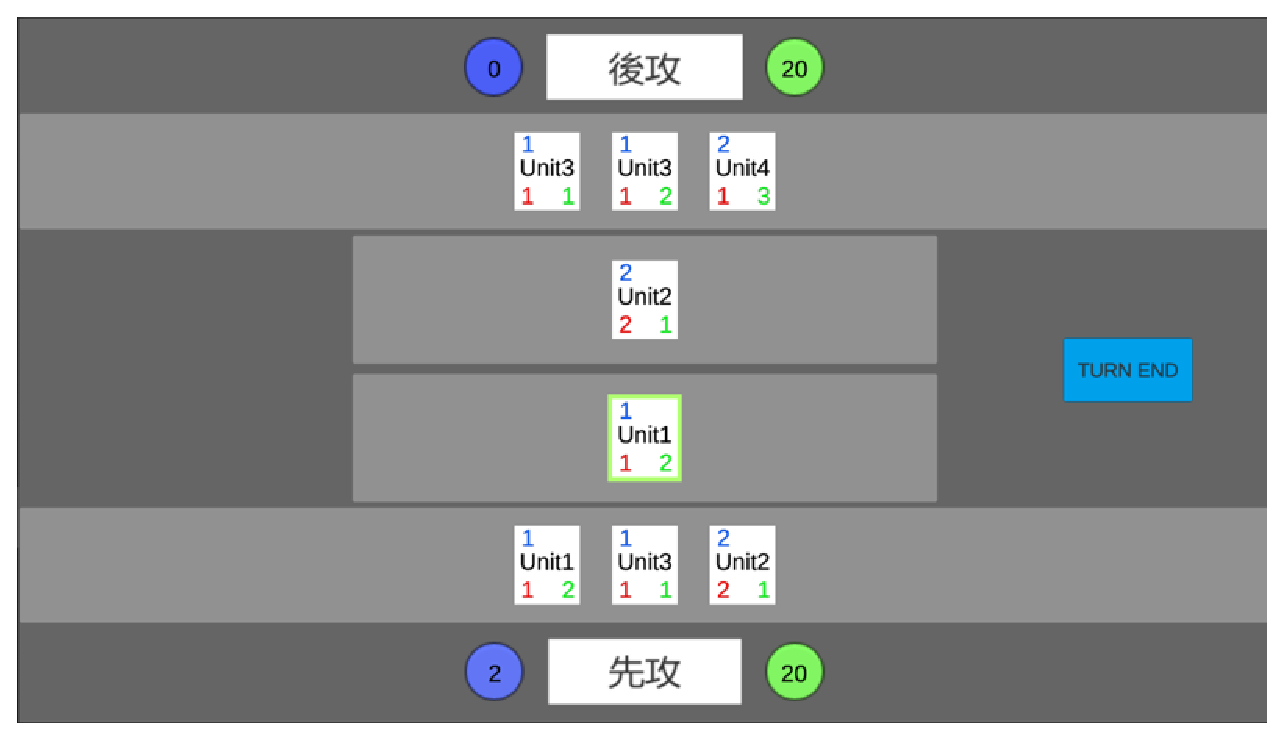
\includegraphics[width=170mm]{assets/cardgamedemo.eps}
  \vspace{-0.3cm}
  \caption{ゲームエンジン Unity で作成した TCG 環境イメージ画像}
  \label{fig:CardGameDemo}
\end{figure}
\subsubsection{プレイヤー}
一般的な TCG と同様に, ゲームは 2 人のプレイヤーからなり, プレイヤーは複数のカードからなるデッキを持つ. 
プレイヤーは手札, 盤面と呼ばれるカードを保有する領域を持ち, ドローと呼ばれる操作でカードをデッキから手札に加える. また, プレイと呼ばれる操作でカードを手札から盤面に出す. また, デッキからカードが無くなった状態をデッキ切れと呼ぶ.  
また, プレイヤー自身が HP, マナという 2 つの整数値パラメータを持つ.
プレイヤー自身の HP が 0 となればゲーム敗北となり, 相手のカードからの攻撃などで減少していく.
マナはカードをプレイする際, 後述するカードのコスト分減少する. プレイヤーは残りマナを超えるコストを持つカードをプレイすることができない. 
今回の環境ではプレイヤーの HP の最大値は 20, マナの上限値は初期値が 1 で最大値を 5 と設定した.
\subsubsection{カード}
カードはそれぞれ攻撃力と HP とコストの 3 つの整数値パラメータを持つ.  盤面にあるカードは対戦相手の盤面にあるカード, あるいは相手プレイヤーに攻撃することができる. カードが攻撃する際には, 相手盤面に存在する攻撃対象のカードの HP, あるいは相手プレイヤーの HP へとカードの持つ攻撃力分ダメージを与える. またカードへと攻撃する際には攻撃対象のカードが持つ攻撃力分, 攻撃するカードもダメージを受ける.
ただし, 攻撃が可能となるのはカードが盤面にプレイされたターンの次のターンからになる. 
カードの HP が 0 になった, あるいは後述する手札と盤面の枚数制限を超えて盤面にプレイされた時はカードは破壊される. 破壊されたカードはゲームから取り除かれる. 
また, カードによっては以下に示す特殊効果を持つものもある.

\begin{description}
  \item[召喚 :]  盤面に出したら (攻撃力 , HP) = (1 , 1) の
  ユニットを追加で盤面に出す
  \item[治癒 :]  盤面に出したら自プレイヤーの HP を 2 回復する
  \item[攻撃 :]  盤面に出したら敵プレイヤーの HP を 2 減らす
  \item[取得 :]  盤面に出したら自プレイヤーは 1 枚カードをドローする
  \item[速攻 :]  盤面に出たターンに攻撃できる
\end{description}

\subsubsection{ゲームの流れ}
以下, ゲームの流れを説明する.
\begin{enumerate}
  \setlength{\itemsep}{0cm} % 項目間
  \item ゲーム開始時に各プレイヤーは自身のデッキをシャッフル.
  \item デッキから初期手札としてカードを 5 枚ドロー. 
  \item 先攻プレイヤーは 1 ターン目のドローステップをスキップし行動.
  \item 後攻プレイヤーはカードを 1 枚ドローして行動.
  \item 2 ターン目以降は先攻プレイヤーもカードを 1 枚ドローしてから行動. 
  \item 4 , 5 の繰り返し. なお, ターンプレイヤーは行動前にマナを上限値まで回復. このときマナの上限値が 5 でなければ上限値を 1 増やしてから回復.
  \item プレイヤーがデッキ切れになっている状態でカードをドローしようとした, あるいはプレイヤー自身の HP が 0 となった場合はそのプレイヤーが敗北となりゲーム終了.
\end{enumerate}
\par
本構築環境では一般的な TCG と同様にカードがプレイされた次のターンから行動可能となるため, 先攻プレイヤーがカードの行動が早くなり有利となる.そのため, 先攻の 1 ターン目のドローステップをスキップしている. 



\subsection{提案手法 2 : DQN によるデッキ内のカードパワーの定量的な評価方法}
TCG においてデッキ内の各カードのカードパワーを測る指標として一般的なものはカードの HP を h, 攻撃力を a, コストを c とすると $\frac{(\mathrm{h} + \mathrm{a})}{2\mathrm{c}} $ として数値化されるマナレシオがある. 
しかし, マナレシオはそのカードの数値のみ HP, 攻撃力, コストの 3 つのみを考慮しており, カードの特殊効果といった指標を考慮していないためあくまで目安にしかならない. \par
本研究では, TCG 環境において DQN を用いた定量的なカードパワー評価指標を提案する.
具体的には, まず DQN を用いてカードパワーを測定したいデッキにおける妥当な戦略を持つエージェントを構築する. 
そしてそのエージェント同士を先攻後攻両方に配置し, 先攻後攻ごとにそれぞれ 1 種類ずつカードを除いて勝率を計算する. これによりデッキ内のカードの種類数 $n_{card}$ について, $n_{card}^2$ 個の勝率の値を得ることができ, これらの値から定量的に構築戦略下のカードパワーを評価する. 


\subsection{提案手法3 : 調整するカード枚数を最小限に抑えた TCG 環境のゲームバランス最適化手法}
本研究では, TCG 環境においてデッキ間の勝率が $50\%$ に近いことがゲームバランスとして好ましいと判断した. 本研究では, 提案手法 2 によってデッキ内のカードパワーを測定し, デッキ内で調整するべきカードの優先順位を定義し, その優先順位に沿って調整するカード枚数を限定して解空間の次元が削減された GA を用いる TCG 環境の最適化手法を提案する. 

\subsubsection{関連研究}
\label{hearthstone}
TCG 環境のゲームバランス最適化タスクをカードのパラメータを対象とした離散値最適化問題と捉えて GA を適用するアプローチはすでに研究されている.
Fernando らは HearthStone \footnote[2]{https://hearthstone.blizzard.com} という TCG 環境内においてデッキ間の勝率が 50 \% となるように, 3 つのデッキの計 64 枚のカードにおける 180 個の調整可能なパラメータを 180 個の要素を持つ 1 次元配列として GA を適用した\cite{EvolvingHearthStone}.
デッキ間の勝率を最適化する単目的 GA を用いた場合, デッキ間の勝率をほぼ 50 \% に近づけるという目標は達成したが, 180 個の調整可能パラメータの総変更量は 402 となり元のデッキの原型が無くなった. 
ゲームバランス最適化の過程において, あまりにもパラメータの変更量が多いとユーザーやゲーム開発者へ与える影響が大きい. そのため多目的 GA である NSGA-II を用いてパラメータの変更量とデッキ間の勝率を目的関数として最適化した.
NSGA-II において, 勝率は GA を用いた場合とほぼ変わらず, パラメータの総変更量は 402 から 154 へと減少し, カードのパラメータ
\par
しかし, NSGA-II を用いることで GA に比べてカードのパラメータの総変更量は減少したが, 変更を及ぼす領域は調整対象のカード全体に及んでいる.  


\subsubsection{提案手法 3 の説明}
提案手法 3 は, TCG 環境のゲームバランス最適化の過程においてパラメータの変更量を抑えるのではなく調整されるカードの枚数を抑えた方が, ゲームの開発者やユーザーにとって好ましいと考え, パラメータの総変更量より「調整されるカード枚数」を抑えた TCG 環境の最適化に着目した.
 具体的には, 提案手法 2 によって得られたカードパワーの評価からデッキにおいて調整されるカードを限定し GA の解空間の次元を削減することで, 直接的に調整されるカードの数を減らす手法を提案する.

\clearpage
\section{実験方法}
独自の TCG 環境下において以下の 3 種類の数値実験をして提案手法の有効性を確かめた.
\subsection{実験 1}
構築したトレーディングカードゲーム環境へ深層強化学習を適用する. 
深層強化学習手法として DQN を用いて構築環境において後攻のプレイヤーとして学習し, 学習済のエージェントで 10000 回ゲームを実行して勝率を計算した. また, 学習側のプレイヤーにデッキには恣意的に弱いカード, 強いカードを 1 種類ずつ追加したデッキを持たせている. 表 \ref{table:OPdeck} にデッキの内容を示す. 表 \ref{table:OPdeck} において, ID が 0 のカードが強いカード, ID が 14 のカードが弱いカードとして恣意的にデッキへ追加したカードである.

\begin{table}[ht]
  \centering
  \caption{学習側のプレイヤーのデッキ}
  \label{table:OPdeck}
  \vspace{-0.3cm}
  \scalebox{0.70}[0.70]{
    \begin{tabular}{|c|c|c|c|c|c|}
      \hline
      ID & 攻撃力 & HP & コスト & 特殊効果 & 枚数 \\ \hline
      0 & 4 & 4 & 1 & 無し & 2 \\ \hline
      1 & 2 & 2 & 2 & 無し & 2 \\ \hline
      2 & 3 & 3 & 3 & 無し & 2 \\ \hline
      3 & 4 & 3 & 4 & 無し & 2 \\ \hline
      4 & 5 & 4 & 5 & 無し & 2 \\ \hline
      5 & 2 & 2 & 2 & 召喚 & 2 \\ \hline
      6 & 2 & 3 & 3 & 召喚 & 2 \\ \hline
      7 & 1 & 1 & 1 & 取得 & 2 \\ \hline
      8 & 1 & 3 & 2 & 取得 & 2 \\ \hline
      9 & 2 & 1 & 2 & 速攻 & 2 \\ \hline
      10 & 3 & 1 & 3 & 速攻 & 2 \\ \hline
      11 & 1 & 2 & 2 & 攻撃 & 2 \\ \hline
      12 & 2 & 3 & 3 & 攻撃 & 2 \\ \hline
      13 & 1 & 1 & 1 & 治癒 & 2 \\ \hline
      14 & 1 & 1 & 5 & 治癒 & 2 \\ \hline
      \end{tabular}
  }
  
  \end{table}
また, 学習が進み具合を把握するため学習時の獲得報酬の推移を記録した.
さらに学習済エージェントを用いて 50000 回の対戦を実行し,エージェントが選択した行動の総数, 各カードごとのプレイされた総数を記録し学習済エージェントがどのような戦略を構築したか, それが人間から見て合理的な戦略かどうか考察した.

\subsubsection{対戦相手}
学習時, また学習後の対戦は共通して同一の対戦相手を設定した. 
対戦相手の戦略として, TCG における代表的な戦略として挙げられるアグロとコントロールの 2 種類を設定した. アグロとコントロールは様々な解釈がありデッキのカードの構成として定義されることもあるが, 本研究では以下のようにカードの攻撃の際の戦略として定義する. これらの戦略を人力で実装した.  図 \ref{alg_aggro}, \ref{alg_controll} に各戦略の詳細な疑似コードを示す. また, 表 \ref{table:agurodeck}, \ref{table:controlldeck} のように戦略ごとに異なるデッキを持たせている. さらに, 表 \ref{winrate_env} に示すように事前にこれらの戦略同士の対戦の勝率は 50 \% 付近に調整してある. 学習, 学習後の対戦において対戦相手は 1 エピソードごとに確率 1 / 2 でアグロかコントロールかを決定される.

\begin{description}
  \item[アグロ :]  敵プレイヤーへの攻撃を優先しなるべく早くゲームエンドに持ち込む. 
  \item[コントロール :]  相手の盤面のカードの処理を優先し, 長期戦に持ち込む.
\end{description}

\begin{figure}[t]
  \vspace{-0.3cm}
  \begin{algorithm}[H]
    \small
      \caption{
        対戦相手の行動ルーチン (アグロ)
        }
      \label{alg_aggro}
      \begin{algorithmic}[1] 
      \STATE 手札から盤面にカードを出せるだけプレイ (ドロー順が古い方から)
      \FOR{自盤面のカード (プレイ順が古い方から)}
      \IF{敵の盤面にカードが無い}
      \STATE 敵プレイヤーを攻撃
      \ELSE
      \IF{自身の HP が 12 以上}
      \STATE 敵プレイヤーを攻撃
      \ELSE
      \IF{敵盤面に破壊できるカードがある}
      \STATE そのカードを攻撃
      \ELSE
      \STATE 敵プレイヤーを攻撃
      \ENDIF
      \ENDIF
      \ENDIF
      \ENDFOR
      \STATE ターンを終了
      \end{algorithmic}
  \end{algorithm}
  \caption{アグロの疑似コード}
  \end{figure}

  \begin{figure}[t]
    \vspace{-0.3cm}
    \begin{algorithm}[H]
      \small
        \caption{
          対戦相手の行動ルーチン (コントロール)
          }
        \label{alg_controll}
        
        \begin{algorithmic}[1] 
        \STATE 手札から盤面にカードを出せるだけプレイ (ドロー順が古い方から)
        \FOR{自盤面のカード (プレイ順が古い方から)}
        \IF{敵の盤面にカードが無い}
        \STATE 敵プレイヤーを攻撃
        \ELSE
        \IF{自盤面の行動可能なカード全てで敵プレイヤーに攻撃すれば勝利}
        \STATE 敵プレイヤーを攻撃
        \ENDIF
        \IF{(敵盤面カードの総攻撃力)$\:\times \:2.0 \:	\textgreater$ (自盤面カードの総 HP)}
        \STATE 敵プレイヤーを攻撃
        \ENDIF
        \IF{敵盤面に HP が残したまま破壊できるカードがある}
        \STATE そのカードを攻撃
        \ENDIF
        \IF{敵盤面に破壊できるカードがある}
        \STATE そのカードを攻撃
        \ELSE
        \IF {敵盤面カードの総攻撃力$\: \textgreater \:$ 自分の HP}
        \STATE 敵盤面の最も攻撃力が高いカードを攻撃
        \ELSE
        \STATE 敵盤面の最も HP の低いカードを攻撃
        \ENDIF
        \ENDIF
        \ENDIF
        \ENDFOR
        \STATE ターンを終了
        \end{algorithmic}
    \end{algorithm}
    \caption{コントロールの疑似コード}
    \end{figure}

    \begin{table}[htbp]
      \begin{minipage}[c]{0.5\hsize}
        \centering
        \caption{アグロのときのデッキ}
        \label{table:agurodeck}
        \vspace{-0.3cm}
        \scalebox{0.70}[0.70]{
          \begin{tabular}{|c|c|c|c|c|c|}
            \hline
            ID & 攻撃力 & HP & コスト & 特殊効果 & 枚数 \\ \hline \hline
            0 & 1 & 1 & 3 & 無し & 2 \\ \hline
            1 & 1 & 1 & 5 & 無し & 2 \\ \hline
            2 & 3 & 2 & 4 & 無し & 2 \\ \hline
            3 & 2 & 2 & 4 & 無し & 2 \\ \hline
            4 & 1 & 2 & 5 & 無し & 2 \\ \hline
            5 & 1 & 2 & 4 & 召喚 & 2 \\ \hline
            6 & 1 & 2 & 4 & 召喚 & 2 \\ \hline
            7 & 1 & 1 & 4 & 取得 & 2 \\ \hline
            8 & 2 & 5 & 1 & 取得 & 2 \\ \hline
            9 & 4 & 4 & 1 & 速攻 & 2 \\ \hline
            10 & 1 & 1 & 4 & 速攻 & 2 \\ \hline
            11 & 1 & 2 & 3 & 攻撃 & 2 \\ \hline
            12 & 1 & 3 & 5 & 攻撃 & 2 \\ \hline
            13 & 1 & 4 & 1 & 治癒 & 2 \\ \hline
            14 & 1 & 2 & 3 & 治癒 & 2 \\ \hline
            \end{tabular}
        }
      \end{minipage}
      \begin{minipage}[c]{0.5\hsize}
        \centering
        \caption{コントロールのときのデッキ}
        \label{table:controlldeck}
        \vspace{-0.3cm}
        \scalebox{0.70}[0.70]{
          \begin{tabular}{|c|c|c|c|c|c|}
            \hline
            ID & 攻撃力 & HP & コスト & 特殊効果 & 枚数 \\ \hline \hline
            0 & 1 & 2 & 2 & 無し & 2 \\ \hline
            1 & 1 & 3 & 2 & 無し & 2 \\ \hline
            2 & 1 & 2 & 2 & 無し & 2 \\ \hline
            3 & 2 & 2 & 4 & 無し & 2 \\ \hline
            4 & 1 & 4 & 2 & 無し & 2 \\ \hline
            5 & 1 & 1 & 2 & 召喚 & 2 \\ \hline
            6 & 1 & 1 & 3 & 召喚 & 2 \\ \hline
            7 & 1 & 2 & 2 & 取得 & 2 \\ \hline
            8 & 1 & 3 & 3 & 取得 & 2 \\ \hline
            9 & 5 & 5 & 1 & 速攻 & 2 \\ \hline
            10 & 1 & 1 & 2 & 速攻 & 2 \\ \hline
            11 & 1 & 2 & 2 & 攻撃 & 2 \\ \hline
            12 & 1 & 1 & 2 & 攻撃 & 2 \\ \hline
            13 & 2& 2 & 1 & 治癒 & 2 \\ \hline
            14 & 2 & 2 & 2 & 治癒 & 2 \\ \hline
            \end{tabular}
        }
      \end{minipage}
    \end{table}

    
    

        \begin{table}[t]
          \centering
          \caption{10000 回のゲーム実行における先攻の勝率}
          \label{winrate_env}
          \vspace{-0.3cm}
          \scalebox{0.70}[0.70]{
            \begin{tabular}{|c|c|c|}
              \hline
              \diagbox[]{先攻}{後攻}      & アグロ    & コントロール \\ \hline
              アグロ    & 0.5255 & 0.5424 \\ \hline
              コントロール & 0.5121 & 0.5053 \\ \hline
              \end{tabular}
          }
          \end{table}

\subsubsection{状態空間, 行動空間, 報酬の定義}
強化学習では, エージェントの取りうる行動と観測できる状態の空間, 報酬を定義する必要がある. 
TCG ではドローやプレイ, カードの攻撃による破壊といった行動で盤面や手札の枚数が変化する場合があり, 各ステップ時点でそれぞれプレイヤーの取りうる行動の総数が変化し得る. そのため, ステップごとに行動空間の次元数が変化し上手く学習できない問題が生じる. \par
そのため本研究では図 \ref{fig:CardGameImage} に示すように予め手札と盤面の枚数の上限をそれぞれ 9 枚, 5 枚と定め, 手札と盤面に存在するカードに自盤面 1 というように番号をつけ, カードが存在しない場合は状態を 0 とすることで状態空間と行動空間を定義した. 表 \ref{table:state}, \ref{table:action} に状態空間, 行動空間の定義を示す.
なお, ドローやプレイといった操作でカードを追加し枚数の上限を超える場合には追加しようとしたカードを破壊する.
\par
また, 報酬は以下のように設定した.\par
\begin{itemize}
  \vspace{-0.3cm}
  \item 1 ステップ終了後 
  \begin{equation*}
   \mathrm{r} = 0.0  
  \end{equation*}
  \item 1 エピソード終了後
  \begin{equation*}
    \mathrm{r} = 
    \left\{
      \begin{aligned}
          1.0 \quad & (\mathrm{学習プレイヤーの勝利}) \\
          -1.0 \quad & (\mathrm{敵プレイヤーの勝利}) \\
      \end{aligned}
    \right.
  \end{equation*} 
\end{itemize}

\vspace{-0.3cm}
\begin{figure}[t]
  \centering
  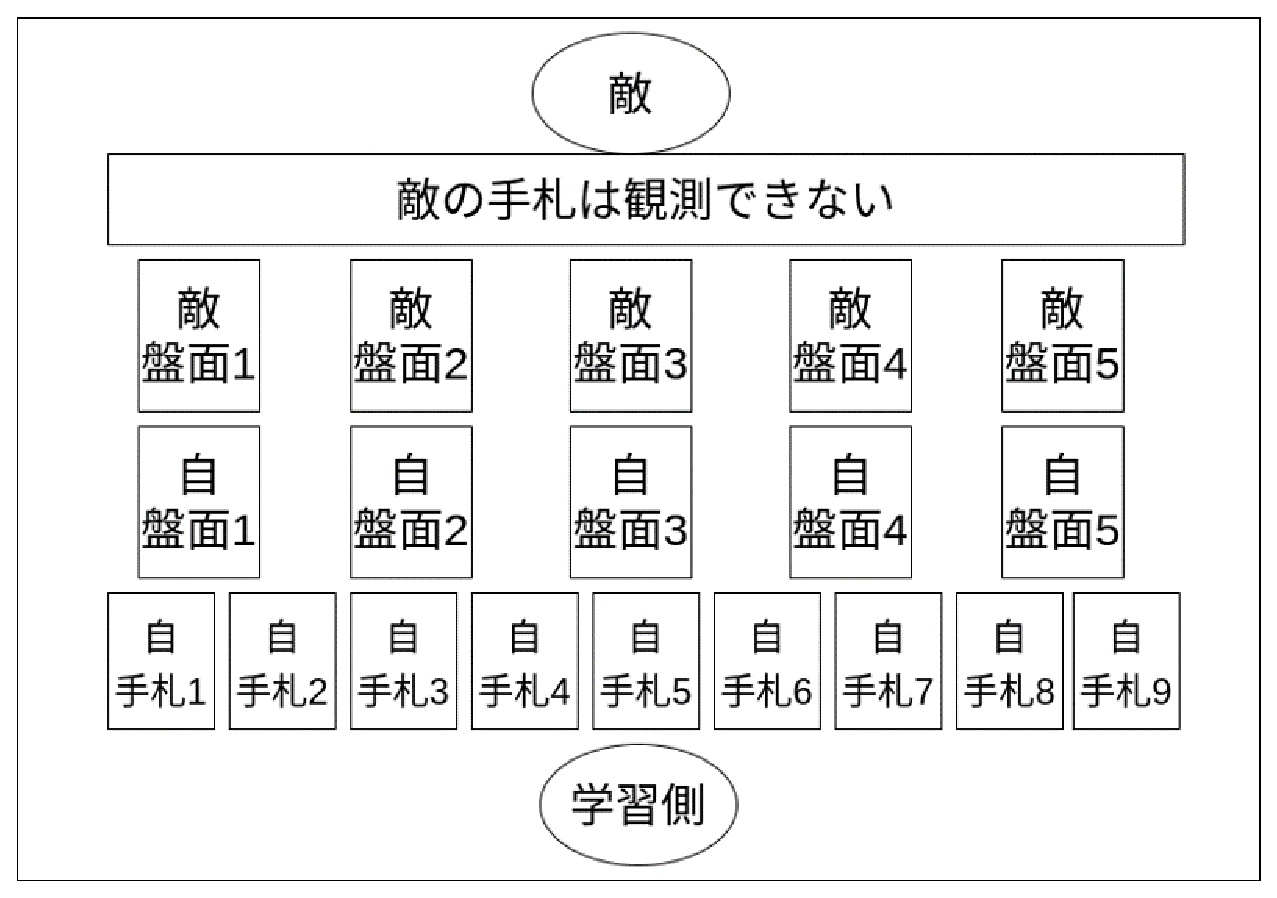
\includegraphics[width=150mm]{assets/cardgameimage.eps}
  \vspace{-0.3cm}
  \caption{深層強化学習における諸定義の際の TCG 環境イメージ}
  \label{fig:CardGameImage}
\end{figure}

\begin{table}[t]
  \small
  \centering
  \caption{定義した状態空間}
  \label{table:state}
  \vspace{-0.3cm}
  \scalebox{0.80}[0.80]{
    \begin{tabular}{|c|c|c|c|}
      \hline
      状態説明                        & 次元数        & 最小値        & 最大値         \\ \hline \hline
      各プレイヤーの HP & 2 & 0 & 20 \\ \hline
      各プレイヤーの マナ & 2 & 0 & 5 \\ \hline
      \begin{tabular}{c}
        手札 1 $\sim$ 9 の\\HP , 攻撃力, コスト, 特殊効果
        \end{tabular}      & 36         & 0          & 5          \\
      \hline
      \begin{tabular}{c}
        自盤面 1 $\sim$ 5 の\\HP と攻撃力
      \end{tabular}     & 10         & 0          & 5 \\
      \hline
      \begin{tabular}{c}
        敵盤面 1 $\sim$ 5 の\\HP と攻撃力
      \end{tabular}     & 10         & 0          & 5 \\
      \hline
      \begin{tabular}{c}
        自盤面 1 $\sim$ 5 が\\攻撃可能かどうか
      \end{tabular} & 5          & 0          & 1  \\
      \hline
      \begin{tabular}{c}
        お互いのデッキの\\残り枚数
      \end{tabular}     & 2 & 0 & 30 \\
       \hline
      \end{tabular}
  }
  \end{table}

  \begin{table}[t]
    \centering
    \caption{定義した行動空間}
    \vspace{-0.3cm}
    \label{table:action}
    \scalebox{0.80}[0.80]{
      \begin{tabular}{|c|c|}
        \hline
        行動説明                          & 次元数        \\ \hline \hline
        手札 1 $\sim$ 9 を自盤面にプレイ             & 9          \\ \hline
        自盤面 1 が敵盤面 1 $\sim$ 5 に攻撃or敵プレイヤーに攻撃    & 6          \\ \hline
        自盤面 2 が敵盤面 1 $\sim$ 5 に攻撃or敵プレイヤーに攻撃    & 6          \\ \hline
        自盤面 3 が敵盤面 1 $\sim$ 5 に攻撃or敵プレイヤーに攻撃    & 6          \\ \hline
        自盤面 4 が敵盤面 1 $\sim$ 5 に攻撃or敵プレイヤーに攻撃    & 6          \\ \hline
        自盤面 5 が敵盤面 1 $\sim$ 5 に攻撃or敵プレイヤーに攻撃    & 6          \\ \hline
        ターンエンド & 1 \\ \hline
        \end{tabular}
    }
      \end{table}

\subsubsection{DQN のパラメータ}

表 \ref{table:dqnparam} に実験 1 で用いた DQN のパラメータを示す.\par
また今回の実験において, ε-greedy における $\epsilon$ は (\ref{epsilon}) 式に従って, $\mathrm{\epsilon_{max}}$ から $\mathrm{\epsilon_{min}}$ へと指数関数的に減少するように設定した. 
\begin{equation}
  \vspace{-0.3cm}
  \label{epsilon}
  \epsilon = \mathrm{max}(\mathrm{\epsilon_{min}} \: , \: \mathrm{\epsilon_{min}} + (\mathrm{\epsilon_{max} - \epsilon_{min}}) \exp(- \frac{\mathrm{n_{step}}}{\mathrm{\epsilon_{decay}}}))
\end{equation}
ここで $\mathrm{n_{step}}$ は学習時の累積ステップを表す. 本実験では $\mathrm{\epsilon_{max}} = 1.0, \mathrm{\epsilon_{min}} = 0.1, \mathrm{\epsilon_{decay}} = 50000$ とした.
\begin{table}[t]
  \centering
  \caption{DQNのパラメータ}
  \vspace{-0.3cm}
  \label{table:dqnparam}
  \scalebox{0.80}[0.80]{
    \begin{tabular}{|c|c|}
      \hline
      パラメータ名 & 値 \\ \hline \hline
      割引率 $\gamma$ & 0.99 \\ \hline     
      全結合層の活性化関数             & ReLU     \\ \hline
      全結合層の次元                & 64       \\ \hline
      最適化アルゴリズム              & Adam     \\ \hline
      方策                 & ε-greedy \\ \hline
      Target Network 更新重み              & 0.5     \\ \hline
      Exprience Memory 開始ステップ数 & $1.0 \times 10^5$ \\ \hline
      学習ステップ数 &  $1.0 \times 10^6$ \\ \hline
      \end{tabular}
  }
  \end{table}

\subsection{実験 2}
実験 2 では実験 1 で構築されたエージェントをそのまま利用する. 
エージェントを先攻後攻両方に配置し, 表 \ref{table:OPdeck} のデッキを両方に持たせる. それぞれデッキからカードを 1 種類ずつ除いて 10000 回対戦を実行し先攻側の勝率を記録する. また比較対象として構築したエージェントだけでなく人力で作成したアグロの戦略を持つプレイヤーにおいても表 \ref{table:OPdeck} のデッキを持たせて先攻後攻両方に配置し, 同様にカードを 1 種類ずつ除いた際の勝率を記録する.

\subsection{実験 3}
TCG 環境に表 \ref{table:OPdeck} のデッキをアグロ用のデッキとして追加し, デッキ間の勝率を 50 \% に近づけるようにゲームバランスを調整するという問題を設定し, 追加するデッキ内のカードのパラメータ (HP, 攻撃力, コスト) を GA を用いて調整した. 表 \ref{winrate_no} にゲームバランス調整をしていない場合の TCG 環境におけるデッキ間の勝率を記録している.
デッキ間の勝率の最適化において, 実験 2 から得られた調整するカードの優先順位を付けて提案手法を適用した. また, 比較手法として関連研究 \cite{EvolvingHearthStone} で用いられた勝率を最適化する単目的 GA および勝率とパラメータの変更量の 2 つを最適化する多目的 GA を適用した.

\begin{table}[t]
  \centering
  \caption{何も調整してない時の先攻の勝率}
  \label{winrate_no}
  \vspace{-0.3cm}
  \scalebox{0.70}[0.70]{
    \begin{tabular}{|c|c|c|c|}
      \hline
      \diagbox[]{先攻}{後攻} &  新追加デッキ (アグロ)    & アグロ    & コントロール \\ \hline
      新追加デッキ(アグロ) & 0.6724 & 0.8005 & 0.8859 \\ \hline
      アグロ &   0.3383  & 0.5255 & 0.5424 \\ \hline
      コントロール& 0.2774 & 0.5121 & 0.5053 \\ \hline
      \end{tabular}
  }
  \end{table}
\subsubsection{GA のパラメータ}
表 \ref{table:gaparam} に GA のパラメータを示す. 
\begin{table}[t]
  \centering
  \caption{GAのパラメータ}
  \vspace{-0.3cm}
  \label{table:gaparam}
  \scalebox{0.80}[0.80]{
    \begin{tabular}{|c|c|}
      \hline
      パラメータ名 & 値 \\ \hline \hline
      世代数 & 50 \\ \hline     
      個体数 & 50     \\ \hline
      遺伝子長 & 調整するカードの種類数 $\times$ 3       \\ \hline
      交叉率 & 0.4 \\ \hline
      交叉の種類 & 2 点交叉 \\ \hline
      個体ごとの突然変異率 & 0.2 \\ \hline
      選択 & 1 個体だけエリート保存, その他はトーナメント方式 \\ \hline
      トーナメントサイズ &  3 \\ \hline
      多目的 GA のアルゴリズム & NSGA-II \\ \hline
      \end{tabular}
  }
  \end{table}

  また, 単目的 GA における適応度, 多目的 GA における目的関数として各解において以下の 3 つの適応度を定義した.
  \begin{itemize}
    \item 適応度 1 : デッキ間の勝率に関する適応度 $f_w$
    \item 適応度 2 : パラメータの変更量に関する適応度 $f_p$
    \item 適応度 3 : 調整されたカード種類数 $f_c$
  \end{itemize}
  GA の各個体について, それぞれの適応度は以下のようにして計算される.\par
  まず, $f_w$ については, 表 \ref{jikken3env} に示される問題設定において, (\ref{f_w}) 式で計算される.
  \begin{equation}
    \label{f_w}
    f_w = \exp(-\sum_{i=0}^4 \sqrt{(0.50 - r_i)^2})
  \end{equation}

  \begin{table}[t]
    \centering
    \caption{実験 3 の問題設定における TCG 環境}
    \label{jikken3env}
    \vspace{-0.3cm}
    \scalebox{0.75}[0.75]{
      \begin{tabular}{|c|c|c|c|}
        \hline
        \diagbox[]{先攻}{後攻} &  新追加デッキ (アグロ)    & アグロ    & コントロール \\ \hline
        新追加デッキ(アグロ) & $r_{0}$ & $r_{1}$ & $r_{2}$ \\ \hline
        アグロ &   $r_{3}$  & 0.5255 & 0.5424 \\ \hline
        コントロール& $r_{4}$ & 0.5121 & 0.5053 \\ \hline
        \end{tabular}
    }
    \end{table}
  また, $f_p$, $f_c$ に関しては, 表 \ref{table:OPdeck} のデッキと解のパラメータ集合を比較してパラメータの変更量 $p$, 調整されたカード種類数 $c$ を計算し, それぞれ (\ref{f_p}), (\ref{f_c}) 式で計算する.
  \begin{equation}
    \label{f_p}
    f_p = \exp(-\frac{p}{200})
  \end{equation}
  \begin{equation}
    \label{f_c}
    f_c = \exp(-\frac{c}{15})
  \end{equation}

\clearpage
\section{結果と考察}
以下, 各実験の結果とその考察を示す.

\subsection{実験 1 : 結果と考察}
表 \ref{table:winratejikken1} に学習後 10000 回対戦を実行し勝率した結果を示す. また, ベースラインとして,後攻に手動で作成した戦略 2 種類を基に行動するプレイヤー, 表 \ref{table:action} に沿ってランダムに行動するプレイヤーを配置し表 \ref{table:OPdeck} のデッキを持たせた際の勝率を示す. 
\begin{table}[ht]
  \centering
  \caption{後攻の戦略を変化させた場合の勝率比較}
  \label{table:winratejikken1}
  \begin{tabular}{|c|c|}
  \hline
  後攻の戦略        & 勝率     \\ \hline \hline
  学習済エージェント    & \textbf{0.7182} \\ \hline
  アグロ          & 0.6914 \\ \hline
  コントロール       & 0.6291 \\ \hline
  表 \ref{table:action} の行動空間に沿ってランダム & 0.2336       \\ \hline
  \end{tabular}
  \end{table}
  これらのベースラインと比べ, 学習済みエージェントは高い勝率を得ていることがわかる. 深層強化学習を用いることで自動的にルールベースで作成した戦略よりも適した戦略を持つエージェントが構築できた.
  図 \ref{fig:jikken1reward} に DQN の学習過程における平均獲得報酬の推移を示す. 横軸が累計エピソード数, 縦軸が報酬の値を表しており, 図の緑点は 500 エピソードにおける報酬の平均値を表しており薄緑の領域は標準偏差を表している. 学習においておよそ報酬の値が 0.0 付近に収束していることがわかる. また, 標準偏差は学習を通して一定のように見える. これは $\mathrm{\epsilon-greedy}$ による定期的な探索によるものと考えられる.
  \begin{figure}[ht]
    \centering
    \includegraphics[width=100mm]{assets/jikken1reward.eps}
    \vspace{-0.3cm}
    \caption{実験 1 における学習中の平均獲得報酬の推移}
    \label{fig:jikken1reward}
  \end{figure}
  
  さらに学習済エージェントで 50000 回対戦を実行し, エージェントが構築した戦略を分析した. 比較対象としては表 \ref{table:winratejikken1} でベンチマークとして用いた表 \ref{table:action} の行動空間に沿ってランダムに行動するエージェントを選んだ. この理由は, 本実験において $\epsilon$ は (\ref{epsilon}) 式に沿って変化し, $\mathrm{\epsilon_{max}} = 1.0$ としたため表 \ref{table:action} の行動空間に沿ってランダムに行動するエージェントは学習最序盤のエージェントとして考えられるためである. これにより学習序盤と学習済のエージェントの戦略の比較ができる.\par
  表 \ref{table:actioncount}に 50000 回の対戦において表 \ref{table:action} の行動空間における各行動でエージェントが選択した総数を示す. 大きな違いとしてランダムの場合はターンエンドが圧倒的に多く選ばれており, 学習済は 2 番目に多い行動とほぼ同数になっている. 表 \ref{table:action} の行動空間の定義ではエージェントが任意にターンエンドを選択できるようになっている. ターンエンドは盤面の状況関係なく常に選択可能な行動であるためランダムの場合は必然的に選択の対象になりうる機会が多い. 学習を進めていくにつれて, まだ行動できるカードが盤面にある, コストが残っておりプレイできるカードが手札にあるといった状況下で無駄なターンエンドをすることが損だと学習していると判断できる. 
  また, 学習済エージェントの行動に着目すると, 盤面のカードは相手の盤面のカードに攻撃することはなく相手プレイヤーに直接攻撃するアグロ寄りの戦略を構築していることがわかる. \par
  表 \ref{table:cardcount} に 50000 回の対戦において各エージェントが表 \ref{table:OPdeck} の各カードをプレイした回数を示す. 表 \ref{table:OPdeck} から, ランダムに行動するエージェント, 学習済みエージェント共にコストが小さいカードほど多くプレイされていることがわかる. ここで, 恣意的にカードを追加した ID 0, 13, 7 のコスト 1 帯のカードと, ID 14, 4 のコスト 5 帯のカードに注目する. ランダムに行動するエージェントではコスト 1, 5 帯において同コスト内でそこまで顕著な差は現れていない. 一方学習済エージェントではコスト 1 帯のカードの中で ID 0 のプレイ回数が明らかに多くなっており, コスト 5 帯のカードの中でID 14 のカードは明らかに少なくなっている. ID 0 は強いカード, ID 14 のカードは弱いカードとして恣意的に追加したカードであるため学習の結果構築戦略下におけるカードの強弱も学習していると考えられる.
  \begin{table}[t]
    \centering
    \caption{選択された総数が多い行動上位 10 個}
    \vspace{-0.3cm}
    \label{table:actioncount}
    \scalebox{0.7}[0.7]{
      \begin{tabular}{|cc|cc|}
        \hline
        \multicolumn{2}{|c|}{ランダム}      & \multicolumn{2}{c|}{学習済}       \\ \hline
        \multicolumn{1}{|c|}{行動説明} & 総数 & \multicolumn{1}{c|}{行動説明} & 総数 \\ \hline \hline
        \multicolumn{1}{|c|}{ターンエンド}    & 401838  & \multicolumn{1}{c|}{ターンエンド}    & 245646  \\ \hline
        \multicolumn{1}{|c|}{手札 4 を盤面にプレイ}    &  92053  & \multicolumn{1}{c|}{手札 1 を盤面にプレイ}    & 213804  \\ \hline
        \multicolumn{1}{|c|}{手札 1 を盤面にプレイ}    & 63841  & \multicolumn{1}{c|}{盤面 1 で相手プレイヤーに攻撃}    & 197221  \\ \hline
        \multicolumn{1}{|c|}{盤面 1 で相手プレイヤーに攻撃}    & 63458  & \multicolumn{1}{c|}{盤面 2 で相手プレイヤーに攻撃}    & 103490  \\ \hline
        \multicolumn{1}{|c|}{手札 2 を盤面にプレイ}    & 61304  & \multicolumn{1}{c|}{手札 2 を盤面にプレイ}    & 68018  \\ \hline
        \multicolumn{1}{|c|}{手札 5 を盤面にプレイ}    & 57697  & \multicolumn{1}{c|}{盤面 3 で相手プレイヤーに攻撃}    & 43093  \\ \hline
        \multicolumn{1}{|c|}{手札 6 を盤面にプレイ}    & 57101  & \multicolumn{1}{c|}{手札 3 を盤面にプレイ}    & 37083  \\ \hline
        \multicolumn{1}{|c|}{手札 3 を盤面にプレイ}    & 51952  & \multicolumn{1}{c|}{手札 4 を盤面にプレイ}    & 22659  \\ \hline
        \multicolumn{1}{|c|}{盤面 1 で相手盤面 1 に攻撃}    & 50430  & \multicolumn{1}{c|}{盤面 4 で相手プレイヤーに攻撃}    & 15419  \\ \hline
     
        \multicolumn{1}{|c|}{盤面 1 で相手盤面 2 に攻撃}    & 41688  & \multicolumn{1}{c|}{手札 5 を盤面にプレイ}    & 15275  \\ \hline
        \end{tabular}
    }
  \end{table}

  \begin{table}[t]
    \centering
    \caption{各カードが盤面にプレイされた総数 (降順)}
    \vspace{-0.3cm}
    \label{table:cardcount}
    \scalebox{0.80}[0.70]{
      \begin{tabular}{|cc|cc|}
        \hline
        \multicolumn{2}{|c|}{ランダム}       & \multicolumn{2}{c|}{学習済}       \\ \hline
        \multicolumn{1}{|c|}{ID} & 総数    & \multicolumn{1}{c|}{ID} & 総数   \\ \hline \hline
        \multicolumn{1}{|c|}{13}  & 35173 & \multicolumn{1}{c|}{0}  & 32965 \\ \hline
        \multicolumn{1}{|c|}{0}  & 35163 & \multicolumn{1}{c|}{13} & 31845 \\ \hline
        \multicolumn{1}{|c|}{7}  & 35068 & \multicolumn{1}{c|}{7}  & 31581 \\ \hline
        \multicolumn{1}{|c|}{11} & 31134 & \multicolumn{1}{c|}{1}  & 26215 \\ \hline
        \multicolumn{1}{|c|}{9} & 30956 & \multicolumn{1}{c|}{11} & 26184 \\ \hline
        \multicolumn{1}{|c|}{1}  & 30672 & \multicolumn{1}{c|}{5}  & 25990 \\ \hline
        \multicolumn{1}{|c|}{5}  & 30401 & \multicolumn{1}{c|}{8}  & 25986 \\ \hline
        \multicolumn{1}{|c|}{8}  & 30386 & \multicolumn{1}{c|}{9}  & 25697 \\ \hline
        \multicolumn{1}{|c|}{12} & 26558 & \multicolumn{1}{c|}{12}  & 21763 \\ \hline
        \multicolumn{1}{|c|}{10} & 26521 & \multicolumn{1}{c|}{2}  & 21560 \\ \hline
        \multicolumn{1}{|c|}{6}  & 25866 & \multicolumn{1}{c|}{6} & 21393 \\ \hline
        \multicolumn{1}{|c|}{2}  & 25700 & \multicolumn{1}{c|}{10}  & 21367 \\ \hline
        \multicolumn{1}{|c|}{3} & 21301 & \multicolumn{1}{c|}{3}  & 19382 \\ \hline
        \multicolumn{1}{|c|}{14}  & 18751 & \multicolumn{1}{c|}{4} & 17639 \\ \hline
        \multicolumn{1}{|c|}{4}  & 18610 & \multicolumn{1}{c|}{14} & 16807 \\ \hline
        \end{tabular}
    }
    \end{table}

\subsection{実験 2 : 結果と考察}
表 \ref{winrate_aguro}, \ref{winrate_agent} に実験 2 の結果を示す. 表の 1 行目と 1 列目はデッキから除くカード ID を表している. また, 表内で表す太字は表内における最大値と最小値である. 
\par
表内の数値は先攻の勝率を表しているため, 表 \ref{winrate_aguro} における最小値からは先攻から ID 0 を除いて後攻から ID 14 を除いた際の先攻の勝率である. このため, デッキにおいて ID 0 のカードが最も強いカード, ID 14 のカードが最も弱いカードと判断できる. 表 \ref{winrate_aguro} における最大値は先攻から ID 14 を除いて後攻から ID 0 を除いた場合であることから同様に判断できる.
\par
このようにして,  表 \ref{winrate_aguro}, \ref{winrate_agent} の結果を比較すると, どちらの戦略においても ID 0 のカードが最も強いカードと判断された一方で, 最も弱いカードに関しては表 \ref{winrate_aguro} では ID 14, 表 \ref{winrate_agent} では ID 8 と戦略によって異なる結果となった.
これは実験 1 の事前学習の効果により, 学習済エージェント同士の対戦において恣意的に弱く設定したカードは登場回数が少なく勝率計算に及ぼす影響が小さかったためであると考えられる. 
表 \ref{table:jikken2cardrecord} にカードを除かない場合でアグロ同士とエージェント同士で 10000 回対戦を実行した場合の各カードにおいて先攻がプレイした総数を記録した結果を示す.
全体的に数値が減少していることから学習済エージェント同士の対決においてはアグロ同士よりも早くゲームが終了していると考えられる.
学習済エージェント同士の対戦においては, 実験 1 で考察したように ID 14 のカードは弱いと学習していると考えられるため ID 14 のカードが勝率へ及ぼす影響がアグロ同士の対戦よりも減少し, 結果としてデッキ内で一番弱いと判断されるカードが異なるカードになったと考えられる.
以上の点から DQN を用いてより人間のプレイに近い戦略下におけるカードパワーを評価できると判断できる. 





\begin{table}[ht]
  \centering
  \caption{アグロ同士におけるカードを 1 種類ずつ除いたときの先攻の勝率}
  \label{winrate_aguro}
  \vspace{-0.3cm}
  \scalebox{0.65}[0.65]{
    \begin{tabular}{|c|c|c|c|c|c|c|c|c|c|c|c|c|c|c|c|}
      \cline{1-16}
      \diagbox[]{先攻}{後攻}                         & 0      & 1      & 2      & 3      & 4      & 5      & 6      & 7      & 8      & 9      & 10     & 11     & 12     & 13     & 14     \\ \hline
      \multicolumn{1}{|c|}{0}  & 0.7857 & 0.4998 & 0.4957 & 0.4779 & 0.4671 & 0.5059 & 0.4914 & 0.5153 & 0.4845 & 0.5105 & 0.5099 & 0.4953 & 0.5128 & 0.5288 & \textbf{0.4335} \\ \hline
      \multicolumn{1}{|c|}{1}  & 0.8955 & 0.6762 & 0.6798 & 0.6688 & 0.6613 & 0.6963 & 0.6789 & 0.6913 & 0.6807 & 0.6925 & 0.6914 & 0.6855 & 0.6998 & 0.6974 & 0.6345 \\ \hline
      \multicolumn{1}{|c|}{2}  & 0.8936 & 0.6763 & 0.6865 & 0.6667 & 0.6652 & 0.6961 & 0.6826 & 0.6850 & 0.6697 & 0.6839 & 0.6864 & 0.6938 & 0.6903 & 0.6958 & 0.6473 \\ \hline
      \multicolumn{1}{|c|}{3}  & 0.9088 & 0.6989 & 0.6939 & 0.6844 & 0.6700 & 0.7119 & 0.6991 & 0.6967 & 0.6932 & 0.7130 & 0.6996 & 0.7061 & 0.7116 & 0.7135 & 0.6599 \\ \hline
      \multicolumn{1}{|c|}{4}  & 0.9049 & 0.7043 & 0.7073 & 0.6816 & 0.6834 & 0.7261 & 0.7109 & 0.709  & 0.7008 & 0.7193 & 0.7173 & 0.7154 & 0.7163 & 0.7269 & 0.6729 \\ \hline
      \multicolumn{1}{|c|}{5}  & 0.8773 & 0.6547 & 0.6635 & 0.6511 & 0.6219 & 0.6721 & 0.6586 & 0.6594 & 0.6451 & 0.6780 & 0.6711 & 0.6682 & 0.6732 & 0.6748 & 0.6211 \\ \hline
      \multicolumn{1}{|c|}{6}  & 0.8929 & 0.6799 & 0.6845 & 0.6701 & 0.6673 & 0.7083 & 0.6795 & 0.6865 & 0.6802 & 0.6988 & 0.6844 & 0.7040 & 0.6925 & 0.7013 & 0.6397 \\ \hline
      \multicolumn{1}{|c|}{7}  & 0.8698 & 0.6539 & 0.6565 & 0.6439 & 0.6317 & 0.6659 & 0.6464 & 0.6602 & 0.6459 & 0.6660 & 0.6637 & 0.6626 & 0.6711 & 0.6750 & 0.6175 \\ \hline
      \multicolumn{1}{|c|}{8}  & 0.9028 & 0.6904 & 0.6897 & 0.6741 & 0.6772 & 0.7063 & 0.7011 & 0.6949 & 0.6793 & 0.7102 & 0.7046 & 0.6954 & 0.7156 & 0.7127 & 0.6621 \\ \hline
      \multicolumn{1}{|c|}{9}  & 0.8762 & 0.6568 & 0.6625 & 0.6549 & 0.6325 & 0.6677 & 0.6630 & 0.6633 & 0.6539 & 0.6782 & 0.6676 & 0.6618 & 0.6792 & 0.6737 & 0.6215 \\ \hline
      \multicolumn{1}{|c|}{10} & 0.8846 & 0.6711 & 0.6716 & 0.6443 & 0.6454 & 0.6883 & 0.6706 & 0.6724 & 0.6609 & 0.6807 & 0.6740 & 0.6744 & 0.6904 & 0.6886 & 0.6242 \\ \hline
      \multicolumn{1}{|c|}{11} & 0.8853 & 0.6671 & 0.6820 & 0.6580 & 0.6484 & 0.6960 & 0.6718 & 0.6843 & 0.6759 & 0.6840 & 0.6797 & 0.6812 & 0.6913 & 0.6862 & 0.6253 \\ \hline
      \multicolumn{1}{|c|}{12} & 0.8738 & 0.6525 & 0.6594 & 0.6407 & 0.6337 & 0.6794 & 0.6553 & 0.6651 & 0.6576 & 0.6708 & 0.6695 & 0.6689 & 0.6729 & 0.6801 & 0.6234 \\ \hline
      \multicolumn{1}{|c|}{13} & 0.8714 & 0.6428 & 0.6570 & 0.6338 & 0.6262 & 0.6751 & 0.6508 & 0.6673 & 0.6456 & 0.6666 & 0.6616 & 0.6673 & 0.6753 & 0.6710 & 0.6153 \\ \hline
      \multicolumn{1}{|c|}{14} & \textbf{0.9296} & 0.7308 & 0.7203 & 0.7199 & 0.6943 & 0.7450 & 0.7287 & 0.7391 & 0.7261 & 0.7400 & 0.7381 & 0.7334 & 0.7456 & 0.7422 & 0.6889 \\ \hline
      \end{tabular}
  }
    \end{table}


  \begin{table}[ht]
    \centering
    \caption{学習済みエージェント同士におけるカードを 1 種類ずつ除いたときの先攻の勝率}
    \label{winrate_agent}
    \vspace{-0.3cm}
    \scalebox{0.65}[0.65]{
      \begin{tabular}{|c|c|c|c|c|c|c|c|c|c|c|c|c|c|c|c|}
        \cline{1-16}
        \diagbox[]{先攻}{後攻}   & 0      & 1      & 2      & 3      & 4      & 5      & 6      & 7      & 8      & 9      & 10     & 11     & 12     & 13     & 14     \\ \hline
        \multicolumn{1}{|c|}{0}  & 0.7596 & 0.5051 & 0.5122 & 0.5104 & 0.5021 & 0.5311 & 0.4947 & 0.5283 & \textbf{0.4861} & 0.5448 & 0.5676 & 0.5159 & 0.5306 & 0.5481 & 0.5106 \\ \hline
        \multicolumn{1}{|c|}{1}  & 0.8537 & 0.6677 & 0.6655 & 0.6576 & 0.6626 & 0.6788 & 0.6496 & 0.6651 & 0.6456 & 0.7019 & 0.6997 & 0.6676 & 0.6826 & 0.6757 & 0.6607 \\ \hline
        \multicolumn{1}{|c|}{2}  & 0.8583 & 0.6637 & 0.6673 & 0.6611 & 0.6664 & 0.6774 & 0.6511 & 0.6785 & 0.6370 & 0.7017 & 0.7097 & 0.6645 & 0.6855 & 0.6889 & 0.6621 \\ \hline
        \multicolumn{1}{|c|}{3}  & 0.8620 & 0.6663 & 0.6663 & 0.6713 & 0.6669 & 0.6776 & 0.6522 & 0.6782 & 0.6422 & 0.7041 & 0.7129 & 0.6790 & 0.6889 & 0.6944 & 0.6746 \\ \hline
        \multicolumn{1}{|c|}{4}  & 0.8690 & 0.6773 & 0.6742 & 0.6757 & 0.6783 & 0.6880 & 0.6569 & 0.6767 & 0.6488 & 0.7153 & 0.7133 & 0.6766 & 0.6937 & 0.6941 & 0.6710 \\ \hline
        \multicolumn{1}{|c|}{5}  & 0.8570 & 0.6508 & 0.6558 & 0.6590 & 0.6596 & 0.6613 & 0.6410 & 0.6562 & 0.6249 & 0.6843 & 0.6881 & 0.6597 & 0.6713 & 0.6749 & 0.6549 \\ \hline
        \multicolumn{1}{|c|}{6}  & 0.8745 & 0.6898 & 0.6743 & 0.6839 & 0.6784 & 0.6969 & 0.6629 & 0.6830 & 0.6605 & 0.7133 & 0.7246 & 0.6965 & 0.6977 & 0.6981 & 0.6857 \\ \hline
        \multicolumn{1}{|c|}{7}  & 0.8442 & 0.6494 & 0.6515 & 0.6373 & 0.6371 & 0.6520 & 0.6277 & 0.6566 & 0.6231 & 0.6755 & 0.6763 & 0.6531 & 0.6572 & 0.6640 & 0.6462 \\ \hline
        \multicolumn{1}{|c|}{8}  & \textbf{0.8836} & 0.7041 & 0.6896 & 0.6863 & 0.6960 & 0.7081 & 0.6855 & 0.7018 & 0.6688 & 0.7285 & 0.7358 & 0.7022 & 0.7078 & 0.7119 & 0.7030 \\ \hline
        \multicolumn{1}{|c|}{9}  & 0.8327 & 0.6403 & 0.6363 & 0.6357 & 0.6371 & 0.6493 & 0.6093 & 0.6422 & 0.5987 & 0.6554 & 0.6706 & 0.6317 & 0.6522 & 0.6456 & 0.6364 \\ \hline
        \multicolumn{1}{|c|}{10} & 0.8392 & 0.6255 & 0.6219 & 0.6179 & 0.6195 & 0.6393 & 0.6100 & 0.6320 & 0.6019 & 0.6616 & 0.6734 & 0.6437 & 0.6487 & 0.6495 & 0.6219 \\ \hline
        \multicolumn{1}{|c|}{11} & 0.8621 & 0.6725 & 0.6688 & 0.6587 & 0.6669 & 0.6754 & 0.6480 & 0.6604 & 0.6306 & 0.6982 & 0.7019 & 0.6603 & 0.6785 & 0.6734 & 0.6570 \\ \hline
        \multicolumn{1}{|c|}{12} & 0.8598 & 0.6553 & 0.6475 & 0.6518 & 0.6594 & 0.6622 & 0.6282 & 0.6538 & 0.6253 & 0.6988 & 0.6972 & 0.6659 & 0.6658 & 0.6676 & 0.6500 \\ \hline
        \multicolumn{1}{|c|}{13} & 0.8261 & 0.6381 & 0.6388 & 0.6340 & 0.6277 & 0.6466 & 0.6195 & 0.6545 & 0.6047 & 0.6688 & 0.6736 & 0.6442 & 0.6545 & 0.6452 & 0.6364 \\ \hline
        \multicolumn{1}{|c|}{14} & 0.8469 & 0.6617 & 0.6608 & 0.6585 & 0.6604 & 0.6768 & 0.6463 & 0.6668 & 0.6254 & 0.6950 & 0.6971 & 0.6680 & 0.6711 & 0.6732 & 0.6698 \\ \hline
        \end{tabular}
    }
    
    \end{table}

    \begin{table}[t]
      \centering
      \caption{戦略ごとに各カードが盤面にプレイされた総数 (降順)}
      \vspace{-0.3cm}
      \label{table:jikken2cardrecord}
      \scalebox{0.80}[0.70]{
        \begin{tabular}{|cc|cc|}
          \hline
          \multicolumn{2}{|c|}{アグロ}       & \multicolumn{2}{c|}{学習済}       \\ \hline
          \multicolumn{1}{|c|}{ID} & 総数    & \multicolumn{1}{c|}{ID} & 総数   \\ \hline \hline
          \multicolumn{1}{|c|}{0}  & 7305 & \multicolumn{1}{c|}{0}  & 4538 \\ \hline
          \multicolumn{1}{|c|}{13}  & 7212 & \multicolumn{1}{c|}{13} & 3742 \\ \hline
          \multicolumn{1}{|c|}{7}  & 7122 & \multicolumn{1}{c|}{7}  & 3662 \\ \hline
          \multicolumn{1}{|c|}{1} & 6643 & \multicolumn{1}{c|}{9}  & 3150 \\ \hline
          \multicolumn{1}{|c|}{9} & 6493 & \multicolumn{1}{c|}{5} & 2920 \\ \hline
          \multicolumn{1}{|c|}{11}  & 6490 & \multicolumn{1}{c|}{11}  & 2894 \\ \hline
          \multicolumn{1}{|c|}{5}  & 6441 & \multicolumn{1}{c|}{1}  & 2812 \\ \hline
          \multicolumn{1}{|c|}{8}  & 6419 & \multicolumn{1}{c|}{10}  & 2639 \\ \hline
          \multicolumn{1}{|c|}{12} & 5759 & \multicolumn{1}{c|}{8}  & 2615 \\ \hline
          \multicolumn{1}{|c|}{10} & 5725 & \multicolumn{1}{c|}{12}  & 2470 \\ \hline
          \multicolumn{1}{|c|}{2}  & 5674 & \multicolumn{1}{c|}{2} & 2357 \\ \hline
          \multicolumn{1}{|c|}{6}  & 5642 & \multicolumn{1}{c|}{6}  & 2211 \\ \hline
          \multicolumn{1}{|c|}{3} & 5357 & \multicolumn{1}{c|}{3}  & 2172 \\ \hline
          \multicolumn{1}{|c|}{4}  & 4925 & \multicolumn{1}{c|}{4} & 1629 \\ \hline
          \multicolumn{1}{|c|}{14}  & 4841 & \multicolumn{1}{c|}{14} & 1514 \\ \hline
          \end{tabular}
      }
      \end{table}
  

\subsection{実験 3 : 結果と考察}
提案手法 3 の数値実験の際にはパラメータを調整するカードの優先度を決定する必要がある.
変更するカードの限定には, 表 \ref{winrate_agent} を用いて, 以下の手順で変更するカードの優先順位を決定する. 
\begin{enumerate}
  \item 表内の最大値,最小値を見て, 最も強いカード, 最も弱いカードを確かめる
  \item その 2 枚において対角線上 (先攻後攻そのカードを抜いた時の勝率) を見て, 何も抜いてない時の勝率と比較し,差の絶対値が大きいカードを変更する優先度が最高のカードとする
  \item 先攻で そのカードを抜いた状態で後攻で何も抜いてない場合の勝率を計算する.
  \item 先攻が優先度最高のカードを抜いた場合の行において, 3 で計算した勝率と差の絶対値を取る. 
  \item 値が大きいほど変更する優先度を高く設定する.
\end{enumerate}
今回の実験においては, お互いに何もカードを除いてない時の先攻の勝率は 0.66532 となったため,  2 で ID 0 のカードが優先度最高のカードとする. 3 において, 先攻が ID 0 のカードを除いて後攻が何もカードを除いていない状況における先攻の勝率は 0.5348 となった. 
このように決定した優先順位はカード ID で表すと, \par
$0 > 8 > 6 > 10 > 4 > 1 > 3 > 14 > 2 > 11 > 13 > 9 > 7 > 12 > 5$ \par
となった. \par
表 \ref{jikken3result} に, この優先順位に沿って調整するカードの種類を 1 種類から 14 種類まで GA による解空間を次元を増やしていってデッキ間の勝率に関する適応度 $f_w$ を最適化する単目的 GA を適用した結果を示す.
調整するカードの種類, すなわち GA の解空間の次元が増えるほど $f_w$ に関して良い値を持つ解が得られている. また, 調整するカード枚数が少ない個体に比べて $f_w$ の値が小さい個体があるが, これは GA の初期収束が起こっていると考えられる.  \par
\begin{table}[t]
  \centering
  \caption{パラメータ変更するカードを増やしながら単目的 GA を適応した結果}
  \label{jikken3result}
  \scalebox{0.80}[0.80]{
    \begin{tabular}{|c|c|c|c|}
      \hline
      限定するカード枚数     & $f_p$ & $f_w$ & $f_c$\\ \hline \hline
      1              & 0.9048         & 0.4805 & 0.9355  \\ \hline
      2           & 0.8607         & 0.5893 & 0.8752 \\ \hline
      3        & 0.8607         & 0.6131 & 0.8187  \\ \hline
      4    & 0.7945         & 0.6339 & 0.7659 \\ \hline
      5 & 0.7334         & 0.6395  & 0.7165 \\ \hline
      6 & 0.6977      & 0.6729  & 0.6703 \\ \hline
      7& 0.6637   & 0.7044  & 0.6271 \\ \hline
      8 & 0.7047 & 0.6837 & 0.5866 \\ \hline
      9 & 0.6505 & 0.7686 & 0.5488\\ \hline
      10 & 0.6250 & 0.7728  & 0.5134\\ \hline
      11 & 0.5169 & 0.7627 & 0.4803\\ \hline
      12 & 0.5326 & 0.8078 & 0.4493\\ \hline
      13 & 0.6005 & 0.8103 & 0.4204\\ \hline
      14 &  0.5220 &  0.8261 & 0.3932\\ \hline
      \end{tabular}
  }
  
  \end{table}
図 \ref{fig:jikken3plot} には比較手法として用いたデッキ間の勝率に関する適応度 $f_w$ を最適化する単目的 GA の最終世代の最も良好な解を緑点, $f_w$ とパラメータの変更量 $f_p$ の 2 つを目的関数として最適化する多目的 GA の最終世代のパレートフロントを赤点, 表 \ref{jikken3result} の中で $f_w$ に関して中間的な値となった解の中で最も $f_c$ の値が小さい解を最も良好な解として青点で示す. 図の縦軸は $f_w$, 横軸は $f_p$ を表している. 

\begin{figure}[t]
  \centering
  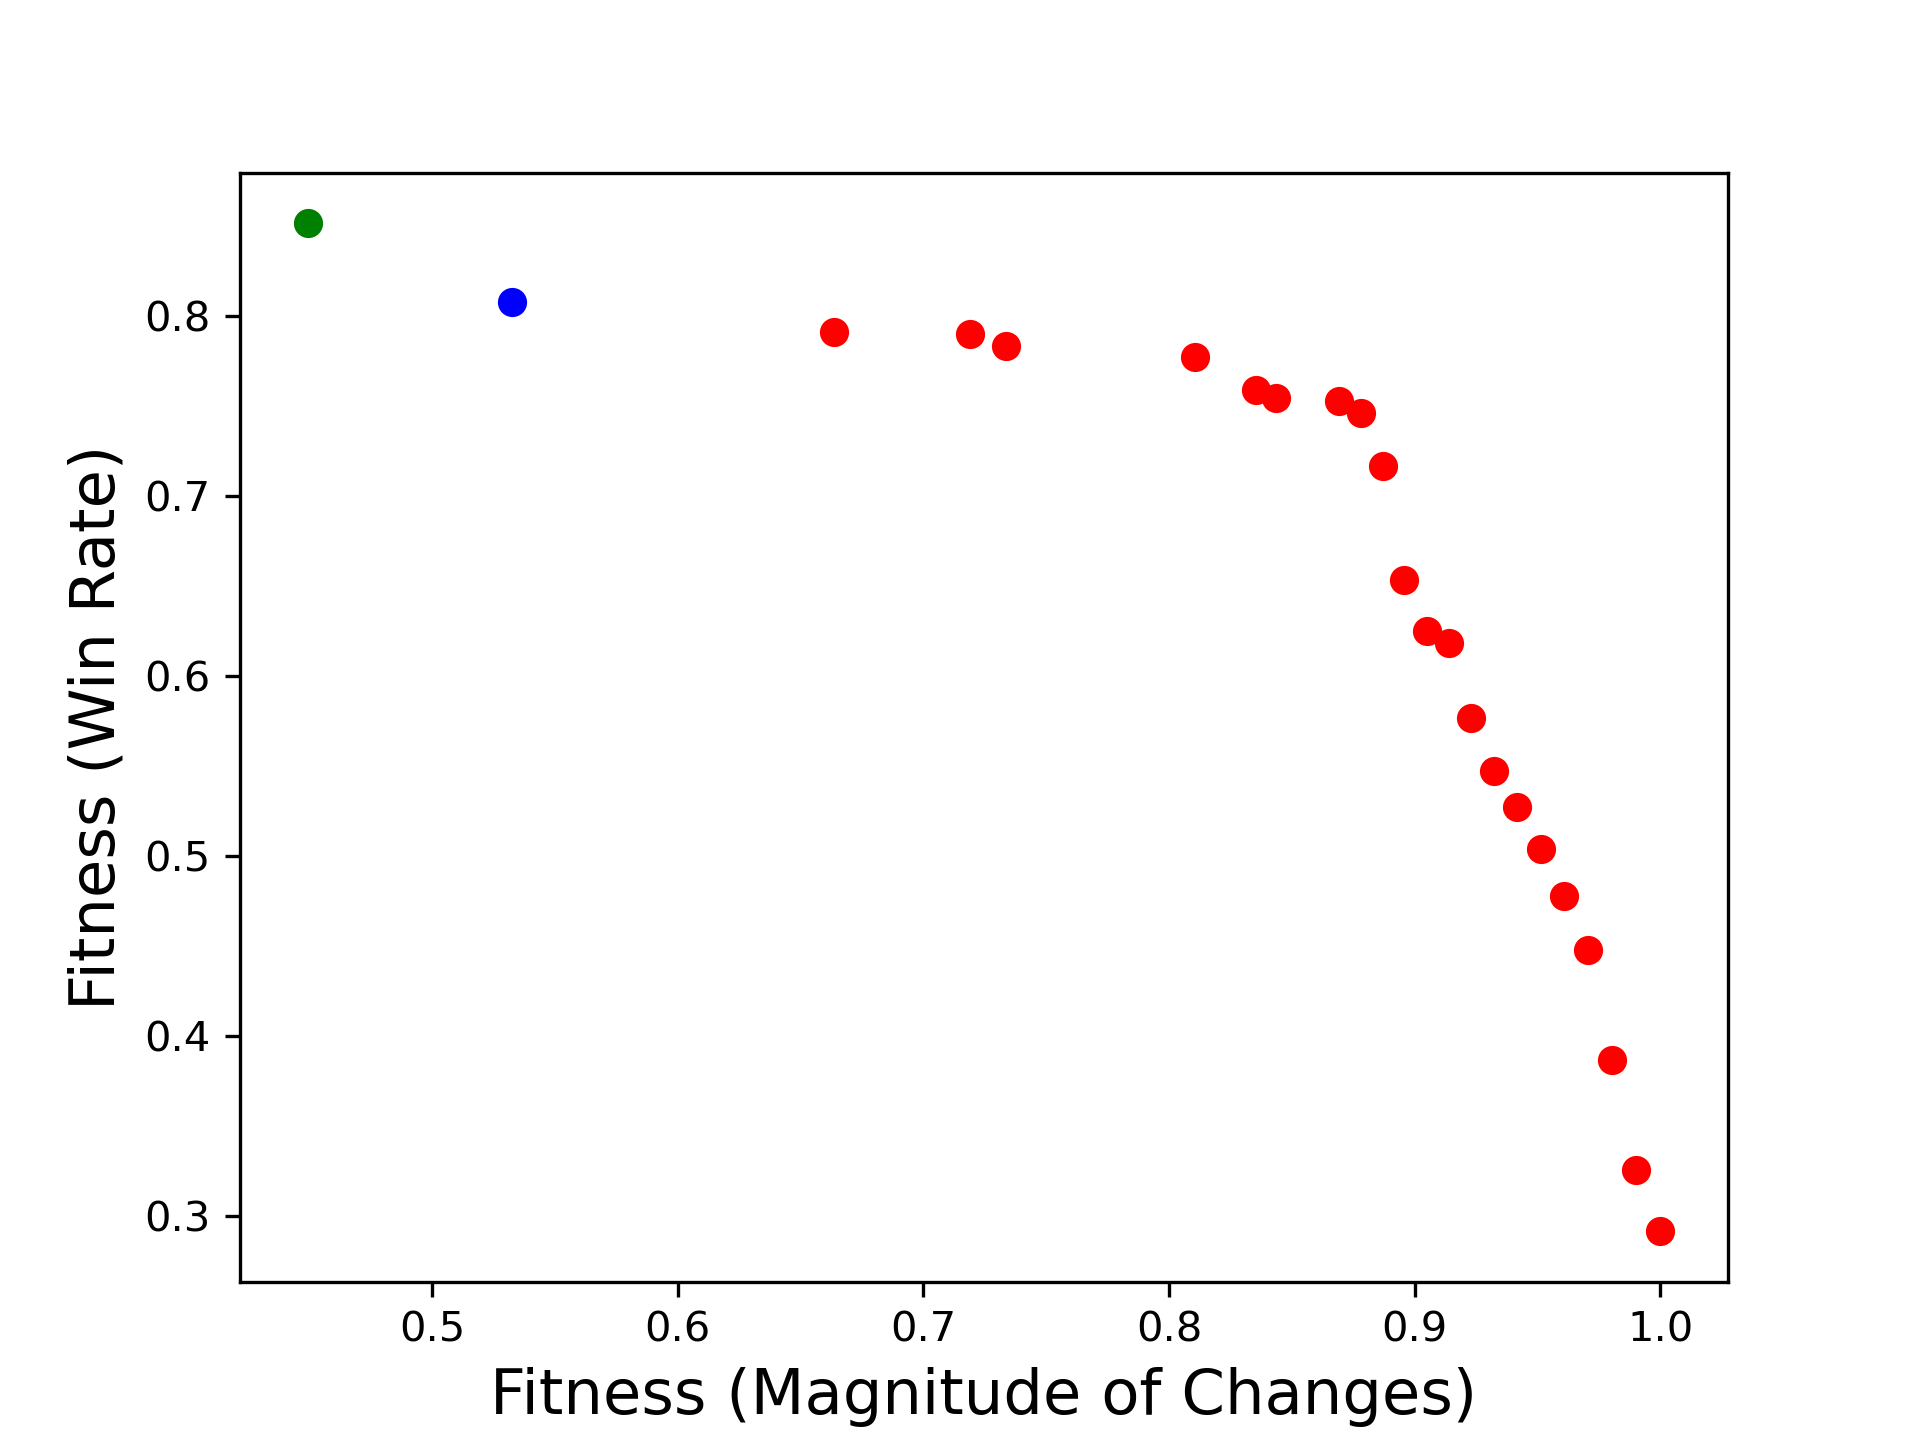
\includegraphics[width=80mm]{assets/jikken3plot.eps}
  \vspace{-0.3cm}
  \caption{提案手法により得られた解と関連研究の最終世代の良好な解}
  \label{fig:jikken3plot}
\end{figure}
図 \ref{fig:jikken3plot} 中の赤点のパレートフロントにおいて $f_p$ の値が最も大きい点を多目的 GA における最も良好な解とする.
表 \ref{res_3} に各手法で得られた最も良好な解の適応度を示す.
\begin{table}[t]
  \centering
  \caption{各手法で得られた最も良好な解の適応度}
  \label{res_3}
  \vspace{-0.3cm}
  
  \scalebox{0.80}[0.80]{
    \begin{tabular}{|c|c|c|c|}
      \hline
      手法        & $f_p$ & $f_w$ & $f_c$ \\ \hline \hline
      単目的 GA      & 0.44933         & \textbf{0.85146}   & 0.36788          \\ \hline
      多目的 GA  & \textbf{0.66365}         & 0.79097   & 0.42035          \\ \hline
      提案手法   & 0.53259              &  0.80783     & \textbf{0.44933}  \\ \hline
      \end{tabular}
  }
  \vspace{-0.3cm}
  \end{table}
各手法において, それぞれの適応度に関して優越した解が得られている. また, 提案手法における最も良好な解は$f_w$ に関して多目的 GA により得られた解に優越しており, $f_c$ に関しては他の手法により得られた解に関して優越している. よって調整されるカードの変更枚数を最小限にする TCG 環境のゲームバランス調整という提案手法 3 の有効性が確かめられた.
\par
各手法において最も良好な解として得られた調整されたデッキの内容を表 \ref{table:monogadeck}, \ref{table:multigadeck}, \ref{table:resultdeck} に示す.
 また, それらのデッキにおける TCG 環境のデッキ間の勝率を表 \ref{winrate_ga}, \ref{winrate_nsga}, \ref{winrate_result} に示す. ゲームバランス調整前の表 \ref{winrate_no} と比べてデッキ間の勝率が 50 \% に近づいていることがわかる. しかし本研究では $f_w$ を (\ref{f_w}) 式のように単純に和で定義しているため, 同デッキ間の勝率は厳密に 50 \% にしたいといった場合には重み付けの和を定義するか異なる定義をする必要があるといえる.

\begin{table}[t]
  \centering
  \caption{単目的 GA により得られたデッキ}
  \label{table:monogadeck}
  \vspace{-0.3cm}
  \scalebox{0.7}[0.7]{
    \begin{tabular}{|c|c|c|c|c|c|}
      \hline
      ID & 攻撃力 & HP & コスト & 特殊効果 & 枚数 \\ \hline \hline
      0 & 3 & 2 & 4 & 無し & 2 \\ \hline
      1 & 5 & 4 & 1 & 無し & 2 \\ \hline
      2 & 1 & 3 & 5 & 無し & 2 \\ \hline
      3 & 1 & 1 & 4 & 無し & 2 \\ \hline
      4 & 2 & 5 & 2 & 無し & 2 \\ \hline
      5 & 1 & 2 & 5 & 召喚 & 2 \\ \hline
      6 & 1 & 1 & 5 & 召喚 & 2 \\ \hline
      7 & 3 & 3 & 5 & 取得 & 2 \\ \hline
      8 & 3 & 3 & 4 & 取得 & 2 \\ \hline
      9 & 3 & 3 & 5 & 速攻 & 2 \\ \hline
      10 & 1 & 2 & 5 & 速攻 & 2 \\ \hline
      11 & 1 & 1 & 5 & 攻撃 & 2 \\ \hline
      12 & 3 & 1 & 5 & 攻撃 & 2 \\ \hline
      13 & 1& 4 & 1 & 治癒 & 2 \\ \hline
      14 & 1 & 5 & 1 & 治癒 & 2 \\ \hline
      \end{tabular}
  }
  
  \end{table}

  \begin{table}[ht]
    \centering
    \caption{多目的 GA によって得られたデッキ}
    \label{table:multigadeck}
    \vspace{-0.3cm}
    \scalebox{0.70}[0.70]{
      \begin{tabular}{|c|c|c|c|c|c|}
        \hline
        ID & 攻撃力 & HP & コスト & 特殊効果 & 枚数 \\ \hline \hline
        0 & 5 & 4 & 1 & 無し & 2 \\ \hline
        1 & 2 & 2 & 4 & 無し & 2 \\ \hline
        2 & 2 & 3 & 5 & 無し & 2 \\ \hline
        3 & 1 & 5 & 4 & 無し & 2 \\ \hline
        4 & 1 & 1 & 5 & 無し & 2 \\ \hline
        5 & 2 & 2 & 5 & 召喚 & 2 \\ \hline
        6 & 2 & 3 & 5 & 召喚 & 2 \\ \hline
        7 & 2 & 1 & 1 & 取得 & 2 \\ \hline
        8 & 2 & 3 & 5 & 取得 & 2 \\ \hline
        9 & 4 & 1 & 5 & 速攻 & 2 \\ \hline
        10 & 3 & 3 & 4 & 速攻 & 2 \\ \hline
        11 & 1 & 3 & 4 & 攻撃 & 2 \\ \hline
        12 & 2 & 3 & 3 & 攻撃 & 2 \\ \hline
        13 & 1 & 2 & 2 & 治癒 & 2 \\ \hline
        14 & 1 & 1 & 5 & 治癒 & 2 \\ \hline
        \end{tabular}
    }
    \end{table}
  
    \begin{table}[ht]
      \centering
      \caption{提案手法において最も良好な解が表すデッキ}
      \label{table:resultdeck}
      \vspace{-0.3cm}
      \scalebox{0.70}[0.70]{
        \begin{tabular}{|c|c|c|c|c|c|}
          \hline
          ID & 攻撃力 & HP & コスト & 特殊効果 & 枚数 \\ \hline \hline
          0 & 1 & 3 & 4 & 無し & 2 \\ \hline
          1 & 4 & 1 & 5 & 無し & 2 \\ \hline
          2 & 2 & 2 & 5 & 無し & 2 \\ \hline
          3 & 2 & 5 & 5 & 無し & 2 \\ \hline
          4 & 4 & 5 & 1 & 無し & 2 \\ \hline
          5 & 2 & 2 & 2 & 召喚 & 2 \\ \hline
          6 & 3 & 1 & 5 & 召喚 & 2 \\ \hline
          7 & 1 & 1 & 1 & 取得 & 2 \\ \hline
          8 & 2 & 1 & 5 & 取得 & 2 \\ \hline
          9 & 1 & 4 & 4 & 速攻 & 2 \\ \hline
          10 & 1 & 4 & 4 & 速攻 & 2 \\ \hline
          11 & 1 & 3 & 5 & 攻撃 & 2 \\ \hline
          12 & 2 & 3 & 3 & 攻撃 & 2 \\ \hline
          13 & 1 & 1 & 4 & 治癒 & 2 \\ \hline
          14 & 1 & 4 & 3 & 治癒 & 2 \\ \hline
          \end{tabular}
      }
      \end{table}
      \begin{table}[t]
        \centering
        \caption{単目的 GA で調整した時の環境における先攻の勝率}
        \label{winrate_ga}
        \vspace{-0.3cm}
        \scalebox{0.7}[0.70]{
          \begin{tabular}{|c|c|c|c|}
            \hline
            \diagbox[]{先攻}{後攻} &  新追加デッキ (アグロ)    & アグロ    & コントロール \\ \hline
            新追加デッキ(アグロ) & 0.5362 & 0.5311 & 0.5678 \\ \hline
            アグロ &   0.5244  & 0.5255 & 0.5424 \\ \hline
            コントロール& 0.4992 & 0.5121 & 0.5053 \\ \hline
            \end{tabular}
        }
        \end{table}

        \begin{table}[ht]
          \centering
          \caption{多目的 GA で調整した時の環境における先攻の勝率}
          \label{winrate_nsga}
          \vspace{-0.3cm}
          \scalebox{0.70}[0.70]{
            \begin{tabular}{|c|c|c|c|}
              \hline
              \diagbox[]{先攻}{後攻} &  新追加デッキ (アグロ)    & アグロ    & コントロール \\ \hline
              新追加デッキ(アグロ) & 0.5814 & 0.5218 & 0.5662 \\ \hline
              アグロ &   0.5613  & 0.5255 & 0.5424 \\ \hline
              コントロール& 0.5211 & 0.5121 & 0.5053 \\ \hline
              \end{tabular}
          }
          \end{table}

          \begin{table}[ht]
            \centering
            \caption{提案手法で調整した時の環境における先攻の勝率}
            \label{winrate_result}
            \vspace{-0.3cm}
            \scalebox{0.70}[0.70]{
              \begin{tabular}{|c|c|c|c|}
                \hline
                \diagbox[]{先攻}{後攻} &  新追加デッキ (アグロ)    & アグロ    & コントロール \\ \hline
                新追加デッキ(アグロ) & 0.5514 & 0.5306 & 0.5441 \\ \hline
                アグロ &   0.5336  & 0.5255 & 0.5424 \\ \hline
                コントロール& 0.5541 & 0.5121 & 0.5053 \\ \hline
                \end{tabular}
            }
            \end{table}
\clearpage
\newpage
\changeindent{0cm}
\section{まとめと今後の課題}

本研究では, 3 つの手法を提案し, 数値実験用の独自の TCG 環境下で数値実験し提案手法の有効性を検証した.
\par
実験 1 では DQN を用いて人力で構築した戦略よりも高い勝率を記録するエージェントを構築した. また, DQN により構築したエージェントはデッキにおいて人間から見ても妥当な戦略を構築しており, 構築戦略下におけるカードの強弱も学習していることが分かった.
\par
実験 2 では提案手法 2 の数値実験をした. 人力で構築した戦略と DQN で構築した戦略では結果に差があった. DQN ではカードの強弱を学習しているためより人間のプレイに近い結果を得られるといえる.
\par
実験 3 では実験 2 で得られた結果を利用して提案手法 3 の数値実験をした. 調整するカード枚数を増やして GA の解空間の次元を増やすほど勝率に関する適応度は高くなっていた. 
また, 提案手法により得られた解は $f_w$ に関しては多目的 GA により得られた解に優越し, $f_c$ については最も優越する解が得られ, 提案手法の有効性が確かめられた.\par
今後の課題を以下に列挙する.
\begin{itemize}
  \item DQN 以外の深層強化学習手法の適用
  \par
  本研究ではエージェント構築の部分に DQN を適用した. 近年では, DQN に様々な工夫を加えた Rainbow \cite{Rainbow}, ターン制完全情報ゲームで顕著な成果を残している AlphaZero \cite{AlphaZero}, その他にも DreamerV2  \cite{DreamerV2}, MuZero \cite{MuZero}, RebeL \cite{ReBeL} など様々な優れた深層強化手法が提案されている. これらの手法を用いることで DQN と比べてより良い戦略を持つエージェントを構築することが期待できる.
  \item GA 以外の最適化手法の適用\par
  本研究では, ゲームバランスの調整においてデッキ内のカードのパラメータを対象として GA を適用した. GA には初期収束という問題がある. GA の選択ルールに熱力学的
  なエントロピーと温度の概念を取り入れることでこれを解決する TDGA \cite{TDGA} を用いることで提案手法 3 においてより良い解が得られると期待できる.
  \newpage
  \item ハイパーパラメータの最適化
  \par
  本研究では, DQN や GA といったアルゴリズムのハイパーパラメータを人力で設定した. Optuna \cite{Optuna} といったハイパーパラメータのチューニングツールを用いて本研究のタスクに適したハイパーパラメータを見つけることでより良い結果を得ることが期待できる.
  \item デッキ間の相性を考慮したゲームバランス調整方法の検討
  \par
  現在はデッキ間の勝率がどの対戦においても勝率が 50 \% に近いほうがゲームバランスとして良い状態としているが, 実際はデッキ間の相性があり, それを事前に推測するメタゲームという概念がある. このような相性まで考慮したバランス調整が重要である.
\end{itemize}




\changeindent{2cm}

%謝辞
\clearpage
\newpage
\changeindent{0cm}
\acknowledgements
\changeindent{2cm}

\begin{flushright}
  年  月  日
\end{flushright}

% 参考文献
\clearpage
\newpage
% \changeindent{0cm}
% \begin{thebibliography}{99}
%  \changeindent{2cm}
%  \bibitem{taro} らてふ太郎, 『LaTeX入門』 https://medemanabu.net/latex/
% \end{thebibliography}


\bibliography{index}
 \changeindent{2cm}
% \bibliography{index}
\bibliographystyle{junsrt} %参考文献出力スタイル


\end{document}